% Chapter Template

\chapter{Question 1 - Password cracking} % Main chapter title

\label{Chapitre 7.1} % Change X to a consecutive number; for referencing this chapter elsewhere, use \ref{ChapterX}

\lhead{ \emph{Password cracking}} % Change X to a consecutive number; this is for the header on each page - perhaps a shortened title

%----------------------------------------------------------------------------------------
%	SECTION 1
%----------------------------------------------------------------------------------------

Ce petit chapitre va nous montrer quelque aspects de la sécurité des mots de passe sur linux. Nous verrons aussi que le mot de passe est directement lié à la technologie utilisée par l'adversaire.

\section{Shadow file}
\subsection{File format}
Le format de ce fichier est comme suit :
\begin{lstlisting}[frame=single,style=Console]  % Start your code-block

username$Ciphersuite$Salt$Hash:lastchanged:minimum_day_between_pass_change:maximum_day_pass_valid:warning_periode_before_pass_expiration:::
\end{lstlisting}

voici quelques explications concernant les différents champs :

\begin{itemize}
\item \textbf{username} : nom d'utilisateur
\item \textbf{Ciphersuite} : suite cryptographique (MD5, SHA512, ...)
\item \textbf{Salt} : Sel ajouté au mot de passe avant le hash
\item \textbf{Hash} : Hash du mot de passe salé 
\item \textbf{lastchanged} : Date du dernier changement
\item \textbf{minimum\_day\_between\_pass\_change} : Temps minimum entre un changement de mot de passe (jours).
\item \textbf{maximum\_day\_pass\_valid} : Temps maximum de validité d'un mot de passe.
\item \textbf{warning\_periode\_before\_pass\_expiration} : Avertissement "n jours" avant l'expiration du mot de passe.\\
\end{itemize}


Pour ce laboratoire nous allons utiliser les suites crytographique MD5 et SHA512

\pagebreak
\subsection{Lab file example}
Voici le fichier "shadow" exemple de 4 utilisateurs test1,test2, test4 et test4 :
\begin{lstlisting}[frame=single,style=Console]  % Start your code-block

test1:$1$9/bUZqUW$Qie8WQyWJVLruS.HVVZsl.:16562:0:99999:7:::
test2:$1$1.ohY/TC$gIfxvKjFx9Ds4E9TIKvO7/:16562:0:99999:7:::
test3:$6$SnW0rDTo$aVhd.akhKipj3jAUBjrSqxYSpMP.hS5qXvitlOIrzGXIHFoJKYTw8YeRRGbh0VJzQYeh2MTwQjJ36BoGs9oyz1:16562:0:99999:7:::
test4:$6$HrOjXB3hsqRAel4/$VKDL6fG4OOWkBp2XlGvu/XQaMRjs.f6v.RDmX1A6aXXH8HYVeOULykT1MNAbvtwl6DAyIQL7AEze2nfX7KyaA0:16562:0:99999:7:::
\end{lstlisting}

Il y a deux mots de passes : "1234" et "Ab\&/3g6S4". Donc un des mots de passe est relativement simple et l'autre est beacoup plus compliqué.
 
\subsection{Using JohnTheRipper}
Nous avons compilé le programme "JohnTheRipper" avec la compatibilité CUDA (GPU Nvidia).

Essayons de lancer le crackage des mots de passe MD5 et SHA512 sur 8 coeurs sans CUDA. Voici les résultats:

(Avec MD5)
\begin{center} 
\hspace{15cm}
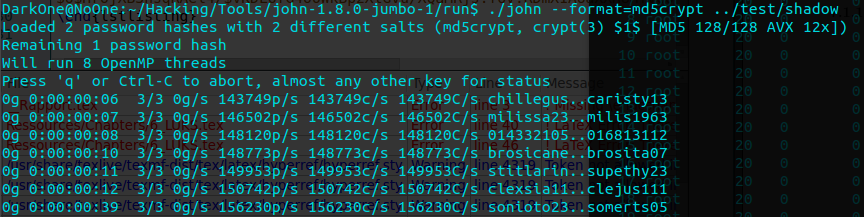
\includegraphics[width=16cm]{JohnCrackMd5.png}
\end{center}
\vspace{0.5cm}

(Avec SHA512)
\begin{center} 
\hspace{15cm}
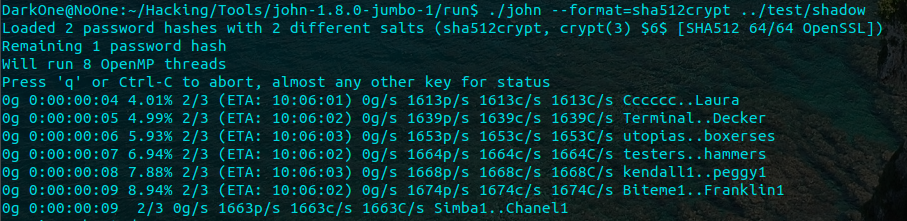
\includegraphics[width=16cm]{JohnCrackSha512.png}
\end{center}
\vspace{0.5cm}

On remarque que l'on passe de 156'230 mots de passe par secondes pour MD5 à 1663 mots de passe par seconde avec SHA512. Ce dernier multiplie presque par 100 le temps pour cracker un même mot de passe.
\pagebreak
 
Le programme à été parrallelisé sur 8 coeurs (d'où les 800\% d'utilisation). Voici la commande "top" :
\begin{center} 
\hspace{15cm}
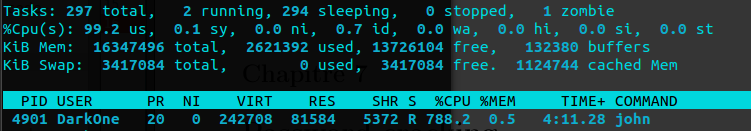
\includegraphics[width=16cm]{TopCrackMd5.png}
\end{center}
\vspace{0.5cm}
 
Voici le résultat retournés :
\begin{center} 
\hspace{15cm}
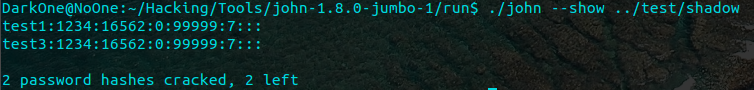
\includegraphics[width=16cm]{JohnCrackedPass.png}
\end{center}
\vspace{0.5cm}

On voit que les mots de passe plus complexes n'ont pas été trouvés. Nous devrions laisser tourner le programme pendant quelques siècles ! Les mots des passes ont été trouvés en un rien de temps (quelques millisecondes à quelques secondes).

\pagebreak
Voici la GPU utilisée est une Nvidia GeForce-870M avec 1344 coeurs CUDA. Ci-dessous les mêmes test effectués cette fois avec la GPU :

(Avec MD5)
\begin{center} 
\hspace{15cm}
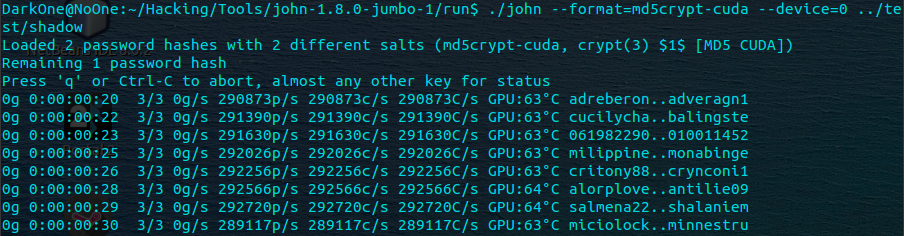
\includegraphics[width=16cm]{JohnCrackCudaMD5.png}
\end{center}
\vspace{0.5cm}

(Avec SHA512)
\begin{center} 
\hspace{15cm}
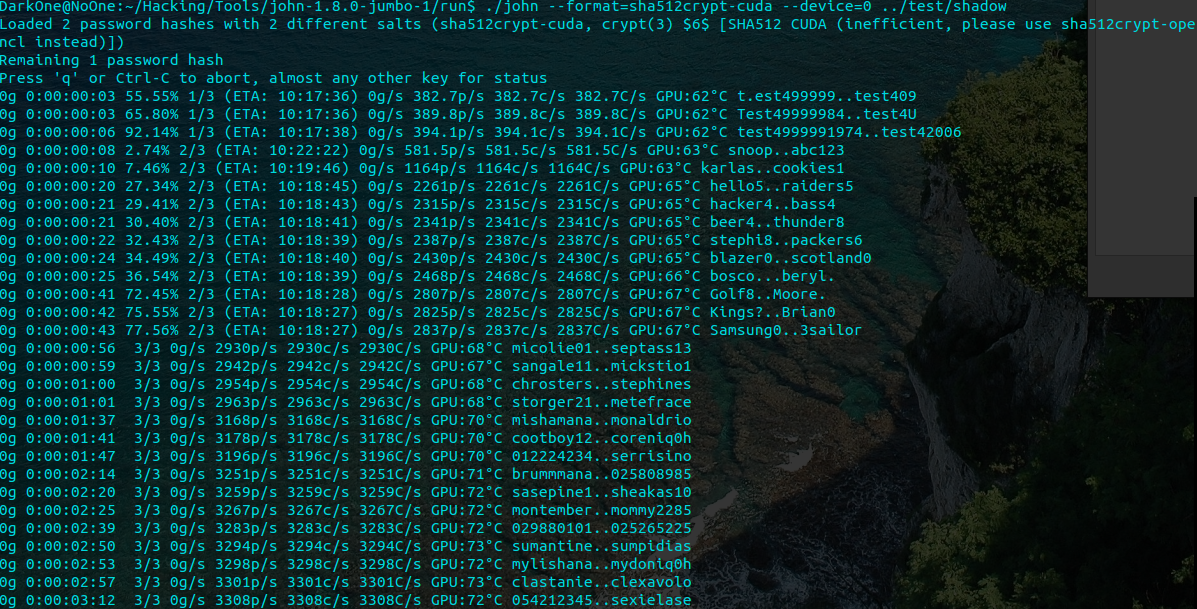
\includegraphics[width=16cm]{JohnCrackSha512Cuda.png}
\end{center}
\vspace{0.5cm}

On voit que pour MD5 on passe de 156'230 p/s à 292'720 p/s, ce qui nous donnes un gain de presque 2. Pour SHA512 on passe de 1663 p/s à 3380 p/s. Au niveau du processeur, on voit que "john" ne consomme presque rien :
\begin{center} 
\hspace{15cm}
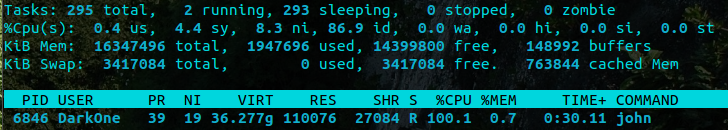
\includegraphics[width=16cm]{TopCrackCudaMD5.png}
\end{center}
\vspace{0.5cm}
